% Le processus d'édition

\section{Édition et édition scientifique}

\subsection{Définition de la notion d'édition}
Le substantif \enquote{édition} est polysémique, mais tous ses sens se rattachent à la notion de diffusion. Le Trésor de la Langue Française informatisé (TLFi) distingue trois grandes significations~: la \enquote{reprodution, publication et diffusion} du livre, la \enquote{préparation du texte d'une \oe{}uvre en vue de sa publication} et, par métonymie des deux premières, le \enquote{texte d'une \oe{}uvre tel qu'il a été fixé par un éditeur} ou le \enquote{texte d'une \oe{}uvre tel qu'il a été publié dans une édition\footnote{Entrée complète sur le site du CNRTL~: \texttt{\href{https://www.cnrtl.fr/definition/edition}{https://www.cnrtl.fr/definition/edition}}.}}.  

L'industrie du livre et de l'édition peut être divisée en deux grands ensembles~: l'édition commerciale et l'édition scientifique. Leur distinction se situe dans le public visé. L'édition commerciale s'adresse, de manière générale, au grand public, tandis que l'édition scientifique s'adresse à un public plus ou moins spécialisé dans un domaine en particulier. Nous ne nous intéresserons dans ce mémoire qu'au volet de l'édition scientifique.  


\subsection{Caractéristiques de l'édition scientifique}
L'historien allemand Patrick Sahle donne la définition suivante d'une édition scientifique~: \enquote{\textit{Edition ist die erschlie\ss{}ende Wiedergabe historischer Dokumente}\footcite[p.~23]{Sahle2016}}. Pour lui, l'essence de l'édition scientifique se trouve dans le sémantisme du verbe \enquote{\textit{erschlie\ss{}en}} (au sens littéral, \enquote{ouvrir} ou \enquote{développer}), mais dont il n'existe pas d'équivalent satisfaisant en anglais (ni, nous le supposons, en français).

Il propose une traduction, en anglais, de sa définition~: \enquote{\textit{A scholarly edition is the critical representation of historic documents}\footcite[p.~23]{Sahle2016}}. Il s'attache ensuite à en définir les termes clés. Il revient, d'abord, sur l'utilisation du terme \enquote{document} plutôt que \enquote{texte}, en déclarant qu'il préfère parler de \enquote{documents} car tous ne contiennent pas que du texte. Nous le rejoignons sur ce point, en particulier dans la mesure où la notion de \enquote{document} nous semble englober celle de \enquote{texte}. Parmi les termes clés, il y a la notion de \enquote{représentation}. Ainsi, la représentation d'un document peut prendre plusieurs formes, telles que sa numérisation ou la transcription de son contenu~; toutefois, pour parler de \enquote{représentation critique}, l'édition se doit d'apporter une information supplémentaire à la simple représentation. L'identification de la structure du document et des entités nommées apporte donc une dimension critique à la représentation d'un document.  

En outre, une édition scientifique a un objectif particulier, celui de \enquote{fournir à la recherche des sources fiables, lisibles, explicitées par une mise en contexte et l'annotation appropriée} et de \enquote{rassembler des corpus éclatés\footcite[p.~19]{NougaretParinet2015}}. C'est précisément cet objectif qui caractérise les éditions en ligne de l'EHRI.



\section{Édition et édition numérique}

\subsection{Caractéristiques d'une édition numérique}
Nous l'avons vu, la distinction entre une édition commerciale et une édition scientifique tient en partie au public auquel elle s'adresse. L'édition numérique, elle, peut être commerciale ou scientifique. Elle s'oppose à l'édition imprimée, notamment au niveau de sa portée.  

Il existe plusieurs façons de publier une édition numérique~: on peut, par exemple, choisir de publier en ligne un ouvrage imprimé sous la forme d'un livre numérique (ou \textit{ebook}), ou bien essayer une forme de publication différente avec un site web. Il a été montré qu'une édition numérique disponible sur Internet sous la forme d'un site web permet une \enquote{démultiplication du public\footcite[p.~314]{Archivistique2020}}. En effet, la fréquentation d'un site web dépasse de loin celle d'une salle de lecture, et une édition numérique publiée en ligne permet de toucher un public international, qui ne pourrait autrement peut-être pas accéder à la ressource qu'il recherche.  

\bigskip
\bigskip
\bigskip
\bigskip
L'édition numérique est particulièrement adaptée pour l'édition scientifique puisqu'elle facilite une lecture non linéaire\footcite[p.~179]{Clavaud2015}. Les nombreux renvois au sein d'une édition, notamment grâce à des liens hypertextes,  facilitent le travail du$\cdot$de la chercheur$\cdot$euse en lui donnant accès d'un simple \enquote{clic} à une référence ou une définition, par exemple.  

Enfin, lorsque l'édition numérique est présentée sous la forme d'un site web, plusieurs \enquote{vues} du document peuvent être proposées. Il est ainsi possible, et grandement pratique, d'afficher à la fois la numérisation du document et sa transcription. Il est également possible de choisir de n'afficher que l'une ou l'autre, ou encore d'opter pour la transcription du texte uniquement ou sa traduction. Les possibilités d'enrichissement pour une édition numérique en ligne sous la forme d'un site web sont nombreuses.


\subsection{Limites de l'édition imprimée}
Chaque mode de publication présente des avantages et des inconvénients. Il faut toutefois reconnaître que certaines caractéristiques de l'édition numérique découlent des limites de l'édition imprimée. Nous nous concentrerons sur deux points qui nous semblent importants~: l'évolution du contenu et le prix.  

La mise en vente d'un livre imprimé marque souvent la fin du travail de l'éditeur$\cdot$ice, à moins de préparer une nouvelle édition. Une édition imprimée représente donc \enquote{une expression figée du travail de l'éditeur\footcite[p.~177]{Clavaud2015}}. La limite de l'édition imprimée se trouve dans la définition du projet éditorial. Une édition d'un texte en particulier bénéficierait d'une édition imprimée, de même que d'une édition numérique sous la forme d'un \textit{ebook}. Au contraire, une édition qui chercherait à mettre à disposition des chercheur$\cdot$euse$\cdot$s de nombreux documents d'archives bénéficierait grandement, voire même uniquement, d'une édition numérique sous la forme d'un site web. En effet, au fur et à mesure des recherches et des découvertes, une édition en ligne peut être augmentée et complétée~:

\begin{quote}
    \enquote{Un site web suffisamment robuste, s'il a été rendu capable d'accueillir à la fois texte et images des documents retenus, pourra en intégrer un nombre très important, ce qui permet notamment d'étendre le périmètre du projet à l'ensemble des reproductions numériques des textes, et finalement à un plus grand nombre de textes qu'une publication imprimée ne pourra en présenter.\footcite[p.~176-177]{Clavaud2015}}
\end{quote}

Cela est particulièrement vrai pour un projet comme les éditions en ligne de l'EHRI, qui sont thématiques~; des archives appartenant à des pays qui rejoindraient l'EHRI dans quelques années pourront intégrer sans problème les éditions déjà publiées.  

Le second aspect qu'il nous paraît important d'évoquer est le prix d'une édition imprimée, notamment pour le$\cdot$la lecteur$\cdot$ice. Se procurer une édition scientifique imprimée peut avoir un coût très élevé\footcite[p.~210]{Pierazzo2019}, et parfois relever de l'impossible en fonction du nombre de tirages et/ou de l'exhaustivité du catalogue de sa bibliothèque. En revanche, une édition numérique peut s'inscrire dans une démarche de science ouverte\footnote{On pourra consulter à ce sujet~: \cite{Romary2016}.}, définie ainsi~:

\begin{quote}
    \enquote{La science ouverte est la diffusion sans entrave des résultats, des méthodes et des produits de la recherche scientifique. Elle s’appuie sur l’opportunité que représente la mutation numérique pour développer l’accès ouvert aux publications et – autant que possible – aux données, aux codes sources et aux méthodes de la recherche\footnote{Voir le deuxième plan national pour la science ouverte~: \texttt{\href{https://www.ouvrirlascience.fr/deuxieme-plan-national-pour-la-science-ouverte-pnso/}{https://www.ouvrirlascience.fr/}}.}.}
\end{quote}

D'un point de vue scientifique, nous estimons qu'il est primordial, surtout lorsque l'on édite des documents d'archives qui serviront de \enquote{sources primaires} aux historien$\cdot$ne$\cdot$s, que le résultat de cette édition soit accessible à tou$\cdot$te$\cdot$s.



\section{La chaîne éditoriale}

\subsection{Définition de la chaîne éditoriale}
Pour fonctionner, l'industrie du livre et de l'édition a besoin d'une \enquote{chaîne éditoriale}. Qu'il s'agisse d'une édition commerciale ou scientifique, imprimée ou numérique, la chaîne éditoriale est centrale.  

\begin{quote}
    \enquote{Une chaîne éditoriale ou chaîne d'édition est la suite d'opérations (ou procédé industriel) par lequel un document rédigé par un auteur est transformé en document publiable et publié. Elle consiste à formater le document écrit, à élaborer des modèles de documents, et à effectuer les conversions de fichiers nécessaires. Elle s'occupe également du stockage et de la diffusion des documents\footnote{Wikipédia, \enquote{chaîne éditoriale}~: \texttt{\href{https://fr.wikipedia.org/wiki/chaine_editoriale}{https://fr.wikipedia.org/wiki/chaine\_editoriale}} (visité le 25/08/2023).}.}
\end{quote}  

La chaîne éditoriale est donc le procédé par lequel est produite une version publiable, imprimée ou en ligne, d'un ou de plusieurs documents.  


\subsection{Un exemple : la \textit{pipeline} DiScholEd}
La publication d'une édition en ligne pouvant être significativement différente de la publication d'une édition imprimée, la chaîne éditoriale de cette dernière nécessite quelques ajustements. Nous prendrons l'exemple de la chaîne d'édition (également appelée \textit{pipeline}) de l'application pour la publication en ligne d'egodocuments, DiScholEd\footnote{La chaîne d'édition de DiScholEd est accessible librement sur GitHub~: \texttt{\href{https://github.com/DiScholEd/pipeline-digital-scholarly-editions}{https://github.com/DiScholEd/pipeline-digital-scholarly-editions}}.} (pour \enquote{\textit{Digital Scholarly Editions}}).  

\begin{figure}[h]
    \centering
    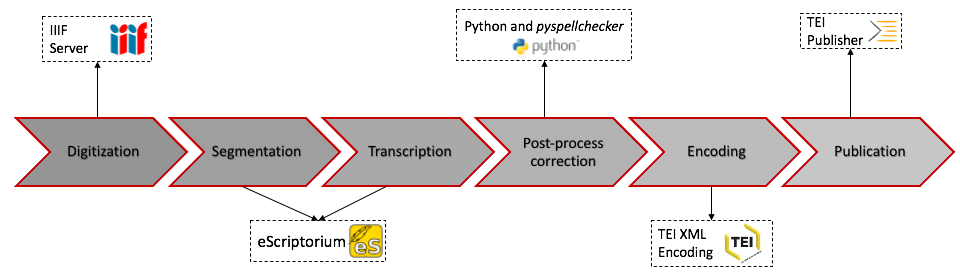
\includegraphics[width=1\linewidth]{2-MAIN//images/pipeline-discholed.png}
    \caption{Chaîne éditoriale de l'application DiScholEd (source~: F. Chiffoleau)}
    \label{fig:pipeline-discholed}
\end{figure}  

La chaîne éditoriale de DiScholEd s'articule actuellement en six étapes. La première étape essentielle est la numérisation. DiScholEd recommande d'héberger les numérisations sur un serveur IIIF\footnote{Pour comprendre le fonctionnement de IIIF~: \texttt{\href{https://iiif.io/get-started/how-iiif-works/}{https://iiif.io/get-started/how-iiif-works/}} (visité le 27/08/2023).}. Le format IIIF est notamment apprécié en raison de son interopérabilité, et du fait qu'il permet la diffusion des images en haute résolution. La transcription d'un document numérisé peut être considérablement accélérée grâce à l'utilisation d'outils de segmentation et de transcription\footnote{DiScholEd recommande l'utilisation d'\textit{eScriptorium}~: \texttt{\href{https://escriptorium.paris.inria.fr/}{https://escriptorium.paris.inria.fr/}} (visité le 27/08/2023).}, basés sur la reconnaissance optique de caractères (OCR) et la reconnaissance d'écritures manuscrites (HTR).

Une fois la transcription vérifiée, il est possible de télécharger un fichier XML de la transcription, prêt à être encodé. Pour cela, il est préférable de suivre les recommandations du standard TEI\footcite{TEIGuidelines}, interopérable et ouvert. L'encodage terminé, le document peut être publié en ligne, sur une plateforme permettant l'affichage de l'encodage sémantique TEI. Notre travail sur les éditions de l'EHRI s'est articulé autour de ces deux dernières étapes de la chaîne éditoriale.  